\documentclass{article}
\usepackage{naturetex}
%如果要中文,写:
\usepackage{ctex}
\renewcommand{\baselinestretch}{1.5}
\usepackage{amsmath}
\usepackage{graphics}
\usepackage{subfigure}
\usepackage{multirow}
\usepackage{float}
\begin{document}

\maketitle

{\setstretch{1.0}
	% *** ABSTRACT ***
	\section*{摘要}
	不可替代代币(NFT) 市场近年来如雨后春笋般涌现。 NFT 的概念最初来源于以太坊的一个代币标准,旨在用可区分的符号来区分每个代币。这种类型的令牌可以与虚拟/数字属性绑定,作为其唯一标识。2021年 NFT 销售的总金额已达到250亿美元。其不断增长的市场的千倍回报引起了全球的广泛关注。然而,NFT 生态系统的发展仍处于初级阶段,NFT 的技术尚不成熟,NFT市场中的定价机制尤为明显。本文试图通过机器学习的方法预测NFT市场的图片价格,进而尝试判断NFT市场中用户的喜好。本研究对于图片的处理方法包括手动提取特征、迁移学习的方法提取特征;在异常值处理方面尝试识别欺诈现象导致的异常价格;使用了基于树的模型获得了模型重要特征。最终模型的拟合结果的$R^2$在0.1左右,测试集的$RMSE$指标在2500左右,模型拟合结果表明影响图片价格的特征包括用户喜好和图片的线条颜色等,同时认为模型拟合效果不好可能和NFT市场本身不够健全有关。
}% setstretch
\newpage 
\tableofcontents
% *** INTRO ***
\newpage
\section{引言}
\subsection{商业背景}
\par 近年来,NFT市场得到快速发展。不可替代代币(NFT)是存储在区块链上的不可互换的数据单元,是一种数字分类账本\cite{wikiNFT},由以太坊的智能合约衍生而来。 NFT 最早是在 Ethereum 改进提案 (EIP)-721 \cite{wang2021non} 中提出的,并在 EIP-1155中得到进一步发展。NFT与比特币等加密货币不同,比特币是一种标准货币,其中所有的货币都是等价且无法区分。相比之下,NFT是独一无二的,不能被同类交换(等效地,不可替代),使其适合以独特的方式识别某物或某人。具体而言,通过使用NFTson智能合约(在以太坊中),创建者可以轻松地以视频、图像、艺术、活动门票等形式证明数字资产的存在和所有权。此外,创作者还可以在任何 NFT 市场或通过点对点交换每次成功交易时赚取版税。完整的历史可交易性、深度流动性和便捷的互操作性使 NFT成为有前途的知识产权(IP)保护解决方案。尽管实际上NFT 仅代表代码,但考虑到其作为数字对象的相对稀缺性,购买者的代码具有归属价值。近年来,NFT 引起了工业界和科学界的极大关注。据悉,NFT 市场 24 小时平均交易量为 4,592,146,914 美元,而整个加密货币市场 24 小时交易量为 341,017,001,809 美元。 NFT 相关解决方案的流动性在5个月内已经占到整个加密货币市场的 1.3\%。早期投资者通过出售独特的数字收藏品获得数千倍的回报。在2021 年 5 月与一年前(2020 年 1 月)相比,NFT 相关市场显著增加。具体而言,销售总数为25,729,完成销售的总金额为34,530,649.86美元。其中一级市场销售总数为17,140,二级销售(用户对用户)的数量为8,589。相应地,一级市场销售使用的美元总额为 8,816,531.10。此外,活跃市场钱包达到 12,836 个,随着时间的推移仍在高速增长。令人惊讶的是,NFT的销售量2020年12月估计为 1200 万,但在短短两个月内(2021 年 2 月)就暴增至 3.4 亿。如此迅猛的发展,让NFT成为了一股热潮,甚至被一些人形容为数字资产的未来。除了以上数据,人们对各种类型的NFT都表达了兴趣,他们热衷于参与NFT相关的游戏或交易。 CryptoPunks\cite{CryptoPunks}是以太坊上最早的 NFT 之一,已经创造了 10,000多个收藏品(6039个男性图标和3840个女性图标),并进一步推动了 ERC-721 标准的流行。 CryptoKitties\cite{CryptoKitties2022Jan} 正式发布 NFT,并在 2017年随着育种机制的游戏化进入市场。参赛者激烈竞价竞拍珍稀小猫,最高价达到 999 ETH3 以上(折合 300 万美元)。
\subsection{研究内容和研究意义}
\par
本文利用机器学习模型预测现有NFT图片商品的价格,进而尝试探究NFT商品的价格关键影响因素,利用这些因素分析当下NFT市场的喜好并给出一定的NFT市场优化建议。NFT销售受多种因素影响\cite{两页NFT价格预测},包括但不限于图片质量、交易者行为和创作者声誉。借助计算机视觉领域的最新发展,可以挖掘NFT 的视觉特征,并对这些图像进行分类、聚类或相似度排序。以通过可能排除潜在偏差来了解是什么使某些 NFT 比其他 NFT更有价值。在图像特征的提取过程中,利用了人工提取特征和卷积神经网络提取特征的方法。其中卷积神经网络 (CNN) 被预测为最适合进行特征提取和可能的图像分类的算法。一些最受欢迎的广泛采用的 CNN如Alexnet和Resnet网络架构可以用在这里,本文利用已经训练好的开源Resnet网络进行学习,进而提取图片特征。另外,尝试特别的方法排除潜在的欺诈行为导致的价格过高。最后使用基于树的模型给出特征的重要性,进而评判哪些特征对于NFT商品的价格是重要的。
\par 本研究是在前人的基础上对NFT定价机制的一次探索。首先,模型本身对于NFT的价格预测有一定的借鉴意义,面对一个商品可以帮助买者确定该商品的价格是否能达到应有的价值,也就是是否有投资意义;另一方面,该模型评价了重要特征,对于NFT的制造者也有重要意义,可以借鉴模型提出的重要特征,从而创作出更加有价值,满足孤苦需求的艺术作品;该模型对于定价机制的研究而言也有着重要价值,鉴于数字资产这个新市场的规模、增长和新颖的规格,这样的研究提供了对早期市场定价行为的重要认识;最后,该模型的研究过程也对于判断市场中是否具有欺诈行为有借鉴意义。

\subsection{现有研究进展}
关于NFT的学术研究还很少。作为一个新兴的研究领域,一个重要的特点是几乎所有现有的论文都对 NFT 进行了简要介绍。论文“Non-Fungible Token (NFT): Overview,Evaluation, Opportunities and Challenges”清晰地解释了 NFT 的基本特征,最初来自以太坊的 ERC-721 协议\cite{wang2021non}。与比特币等传统加密货币不同,基于ERC-721 智能合约的代币具有可区分的符号,不能进行等价交换。在NFT中得到了进一步发展,纳入了 ERC-1155 协议,该协议还集成了 Fungible Tokens (FTs),现已扩展到非以太坊区块链,如 Flow、Wax、Hyperledger、Fast Box 等。 “Mapping the NFT revolution: market trends, trade networks and visual features”\cite{nadini2021mapping}使用 2017 年 6 月 23 日至 2021 年 4 月 27 日期间以太坊和 WAX 区块链上的交易数据探索 NFT 市场的发展路径和表现。结果表明,NFT 的第一个流行例子是 CryptoKitties,它在 2017 年 12 月造成了以太坊网络的阻塞,并促进了 NFT 市场的发展。 NFT 市场规模一直保持稳定,直到 2020 年年中,日均交易量为 6 万美元。自 2020 年 7 月以来,市场经历了快速增长,2021 年 3 月日总交易量超过 1000 万,比 8 个月前增长了 150 倍。对NFT市场的效率和溢出效应的研究是现有论文中最丰富、最具代表性的方向。《Fertile LAND: Pricing non-fungible tokens》选择了最流行的 NFT 应用之一的 Decentraland 来探索 NFT 市场的效率\cite{Dowling2022Jan}。基于 Decentraland 2019 年 3 月至 2021 年 3 月的交易数据,自动方差比(AVR)、自动组合(AP)和 Domínguez 和 Lobato(DL)一致性测试的所有测试证明市场是低效率的,并且有可能是市场操纵或其他Decentraland  定价中的欺诈行为。此外,Lennart Ante 的论文“Non-fungible token (NFT) markets on the Ethereum blockchain: Temporal development, cointegration and interrelations”\cite{ante2021non},探讨了 2017 年 6 月至 2021 年 5 月期间使用来自以太坊区块链的数据的 14 个最大的 NFT 项目的相互作用。同样,《Non-fungible Tokens: Blockchains,Scarcity, and Value》将NFT与加密货币区分开来,将其视为区块链技术更重要的发展方向,进一步挖掘去中心化和分布式账本的潜力。\cite{Fintech2021}
\par 至于现有的NFT商品价格的研究中,集中在2021年才有所发展。Kireyev, Pavel和 Lin等人\cite{kireyev2021infinite}研究了传统的估值方法如何在这个市场上表现出明显的偏差,认为虽然买家对 NFT 的估值就像买家对实物收藏品的估值一样,但卖家倾向于以次优定价,这导致传统的特征回归方法产生不准确的估值,并开发了一种基于流行 NFT市场中使用的销售机制的结构模型的估值方法,以突出这些偏见,从而帮助参与者做出更明智的决策。Nadini, Matthieu和Alessandretti等人\cite{nadini2021mapping}我们分析了来自以太坊等的470 万个 NFT 的 610 万笔交易的数据,通过描述市场的统计特性并建立交互网络,表明了交易者通常专注于与类似对象相关的 NFT,并与交换相同类型对象的其他交易者形成紧密的集群,同时使用简单的机器学习算法研究 NFT 销售的可预测性,并发现销售历史和视觉特征是很好的价格预测指标。这些发现将激发对不同背景下 NFT 生产、采用和交易的进一步研究。
\subsection{探索过程和行文思路}
% TODO: \usepackage{graphicx} required
\begin{figure}[tbph!]
	\centering
	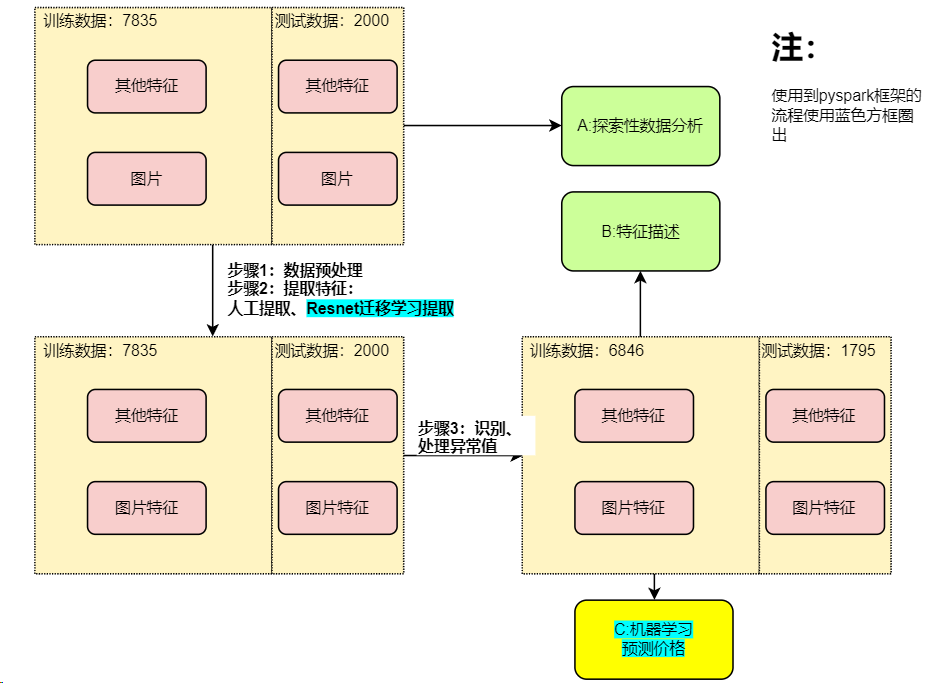
\includegraphics[width=0.7\linewidth]{screenshot001}
	\caption{数据处理思路。主要思路包括特征提取、异常值处理以及探索性数据分析和机器学习,其中蓝色背景的流程使用spark框架进行。}
	\label{fig:screenshot001}
\end{figure}
\par 在本研究中,主要流程如图\ref{fig:screenshot001}所示,其中数据探索主要是对于图片以外的其他特征进行探索;数据的主要处理包括对图片提取特征以及进行异常值检测两个部分;特征描述是对于异常值处理之后的数据进行特征描述;机器学习和特征提取主要使用了pyspark框架。
\par 本文接下来的行文思路如下:
\begin{enumerate}
	\item 数据分析部分主要包括数据预处理和异常值处理两个流程。其中数据预处理对应图\ref{fig:screenshot001}中的步骤1,异常值处理对应图\ref{fig:screenshot001}中的步骤3。另外在探索性数据分析中描述了图片特征以外的特征的探索性分析结论,对应图\ref{fig:screenshot001}中的A。
	\item 预测方法部分主要描述了特征的提取方法、特征的描述以及预测模型构建。其中特征提取方法对应图\ref{fig:screenshot001}中的步骤2,特征描述对应图\ref{fig:screenshot001}中的B。预测模型构建对应图\ref{fig:screenshot001}中的C。
	\item 结论部分描述模型的主要结论以及改进方向。
\end{enumerate}
\section{数据分析}\label{数据分析}
\subsection{数据预处理}
\par 原始数据包括训练集和测试集两部分,训练集包括7835条数据,测试集包括2000条数据,验证集通过训练集的三折交叉验证实现。每条数据包含一张爬取得到的图片以及产品编号、产品类别、产品品牌、产品价格、产品数量、产品受欢迎程度、产品负面信息数量等特征。
\par 首先,对于图片基本描述的数据,删除不相关或无信息的特征,如图片网址、产品id等。
\par 其次,将图片数据处理成特征。发现图片数据比较复杂,一方面,图片的大小不一致,不同的来源的图片可能有不同的像素;另一方面有很多图片是动图格式。这导致了无法直接将图片向量化,另外有研究认为图片向量化之后更不易得到预期希望的结果。为了解决这些问题,对图片进行如下处理:动图图片保留第一帧,其他格式的图片尝试直接进行读取,并将所有读取到的图片缩放为300*300像素的标准图片;所有无法读取的图片进行了删除处理,共留下了7835条训练数据和2000条测试数据。
\subsection{异常值处理}
由于数据来源包含众多市场,异常值也是应该关心的内容。
\par 首先探讨异常值的主要来源。根据现有研究\cite{Dowling2022Jan},NFT领域有抬高物价,价格欺诈等现象,由于在互联网的环境中这种异常的行为很难识别,而且预计这种行为会导致异常数据,即:本身图片并不出众,但依然卖价很高。因此,识别异常值的任务也就变成了寻找价格很高、但本身不出众的图片。
\par 首先假设价格高且不是欺诈行为导致的图片本身应该在其他相应特征上比较出众,即如果利用离群值检测检测合适的特征,那么价格高且正常的商品应该被判定为离群值;同时假设欺诈产生的高价商品在相应特征上不会被视作离群值。如果这种欺诈产生的高价商品在数量上不占多数,也就不会对模型选择重要的、合适的特征产生重大影响。经过以上分析,在此提出具体的处理方法:
\begin{enumerate}
	\item 处理所有商品,获取可能的特征。
	\item 利用模型$M$在训练集上训练,在测试集上做测试,得到表现最好的模型$M_{best}$。
	\item 求得模型$M_{best}$给出的特征重要度$W=[w_1,w_2,...,w_i,...]$
	\item 将重要度乘特征值$W\times Features$得到加权特征值。
	\item 利用加权特征值进行离群值检测,分为离群值组$G_1$和不离群组$G_2$
	\item 不离群组中的所有价格高于离群值组平均值的商品视为异常值,删除。
\end{enumerate}
\par 以上步骤即完成了删除异常值的过程。其中,考虑到模型的训练速度、能够顺利获得特征重要性等问题,预训练的模型选择LightGBM模型。最终异常值删除的过程共删除训练数据989个,删除测试数据205个。
\begin{figure}[!htbp]
	\centering
	\subfigure{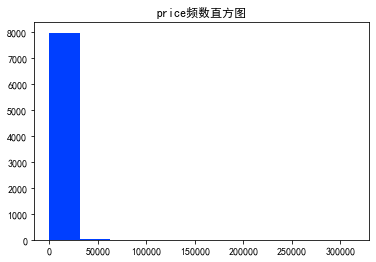
\includegraphics[width=0.4\linewidth]{price频数直方图}}
	\subfigure{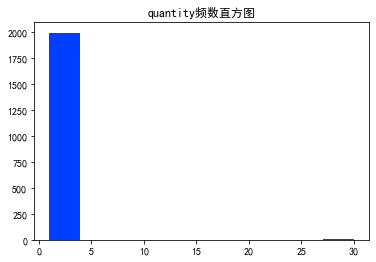
\includegraphics[width=0.4\linewidth]{quantity频数直方图}}
	\subfigure{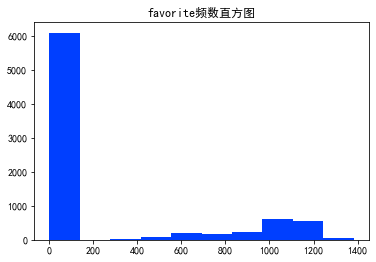
\includegraphics[width=0.4\linewidth]{favorite频数直方图}}
	\subfigure{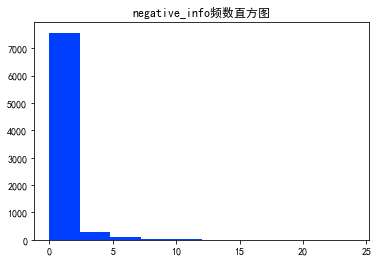
\includegraphics[width=0.4\linewidth]{negative_info频数直方图}}
	\caption{数值型单变量探索性分析。图中展示了数值型变量的频数直方图。}
	\label{图:单变量-频数直方图}
\end{figure}
\subsection{探索性数据分析}
这里主要对图片以外的数据进行探索性数据分析。这些图片以外的数据没有缺失值,另外值得注意的是,价格方面测试集平均价格维1987,训练集平均价格1792,测试集价格高于训练集价格,这可能和测试集不是按照随机分类的原则进行的有关:推测时间更偏后的产品因为NFT市场受到的关注度上升而获得更高的价格;以及随着NFT市场的成熟,出现了炒作商品,推高价格的不正当行为。
\par 其次对所有数值变量绘制频数直方图,可以看到所有数据都呈现右偏分布。price几乎所有的样本价格都在5000以下;quantity几乎所有样本都在0左右;favorite变量呈现在0-100之间和1000-1200之间出现两个高峰,这可能和互联网的曝光的效应有关;负面评价也是在5以下居多,也可能和图片本身因为不引起足够的关注而无法得到有效的负面评价有关。
\par 利用独热编码的方法把product\_id和brand两个分类变量进行编码,绘制箱线图如图\ref{图:单变量-箱线图}所示。其中大部分情况下训练集和测试集样本的均值相差不大,只在产品种类3中测试集平均值更高,产品品牌2和4中测试集平均值更高,这些和测试集本身平均价格高于训练集平均价格有关,而在其他地方价格训练集和测试集相差不明显,说明可能更应该关注这些类别的商品是否有因为炒作推高价格的嫌疑。而在不同种类的商品的比较中,可以看到不同的商品类别有着不同的平均值,比如产品类别2的商品价格普遍高于其他类别,产品品牌2的商品价格普遍高于其他类别。至于出现的离群值,因为不能确定这些离群值产生的原因,在此不做讨论。
\begin{figure}[!htbp]
	\centering
	\subfigure{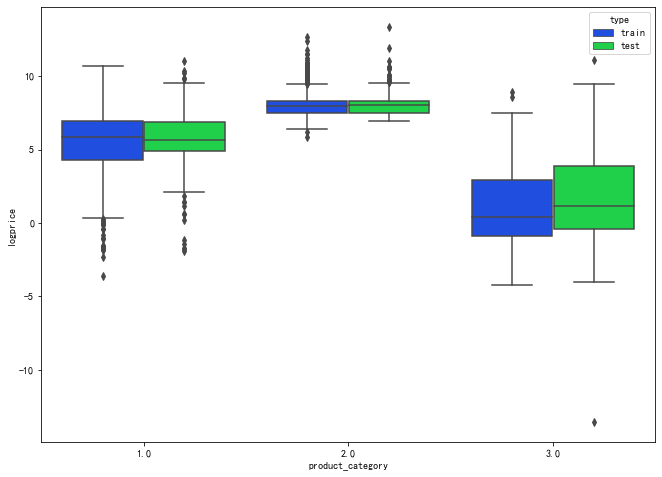
\includegraphics[width=0.4\linewidth]{logprice-产品种类箱线图}}
	\subfigure{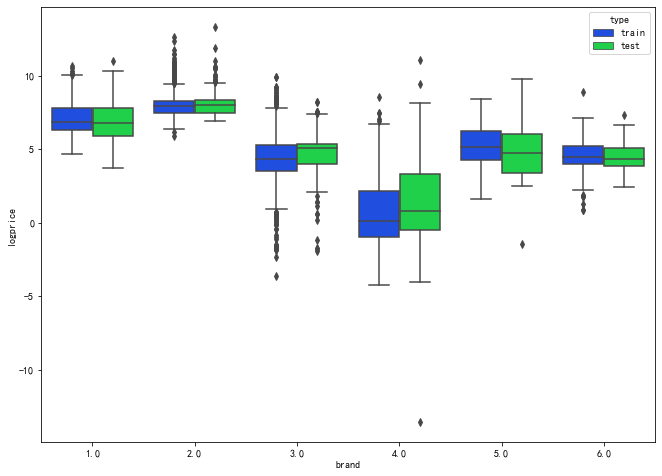
\includegraphics[width=0.4\linewidth]{logprice-品牌箱线图}}
	\caption{类别型单变量探索性分析。图中展示了类别变量的箱线图,其中蓝色箱子代表训练集,绿色箱子代表测试集;横坐标代表不同分类,纵坐标代表对价格取对数之后的值。}
	\label{图:单变量-箱线图}
\end{figure}
\par 为了了解变量之间的相关性,绘制了相关系数矩阵。如图\ref{fig:原变量相关系数矩阵},图中展示出在某些变量之间有着较强的相关性,如品牌1和种类3之间相关性为1。这些高相关性的变量将会在后面删去。

\begin{figure}[!tbph]
	\centering
	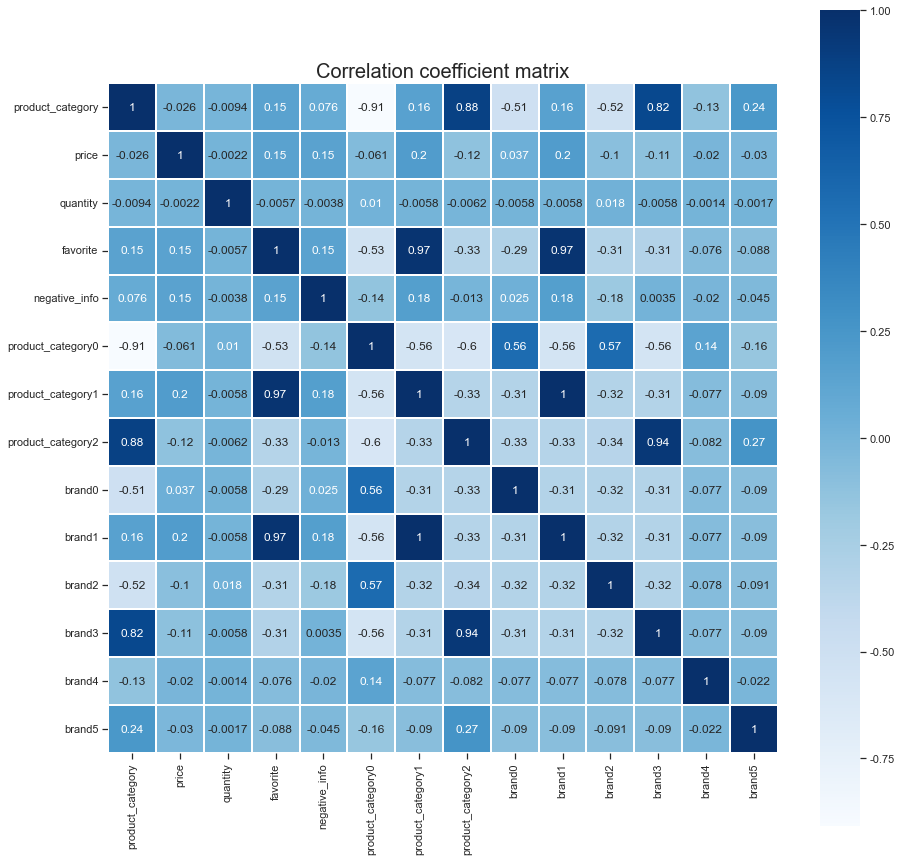
\includegraphics[width=0.45\linewidth]{figures/原变量相关系数矩阵}
	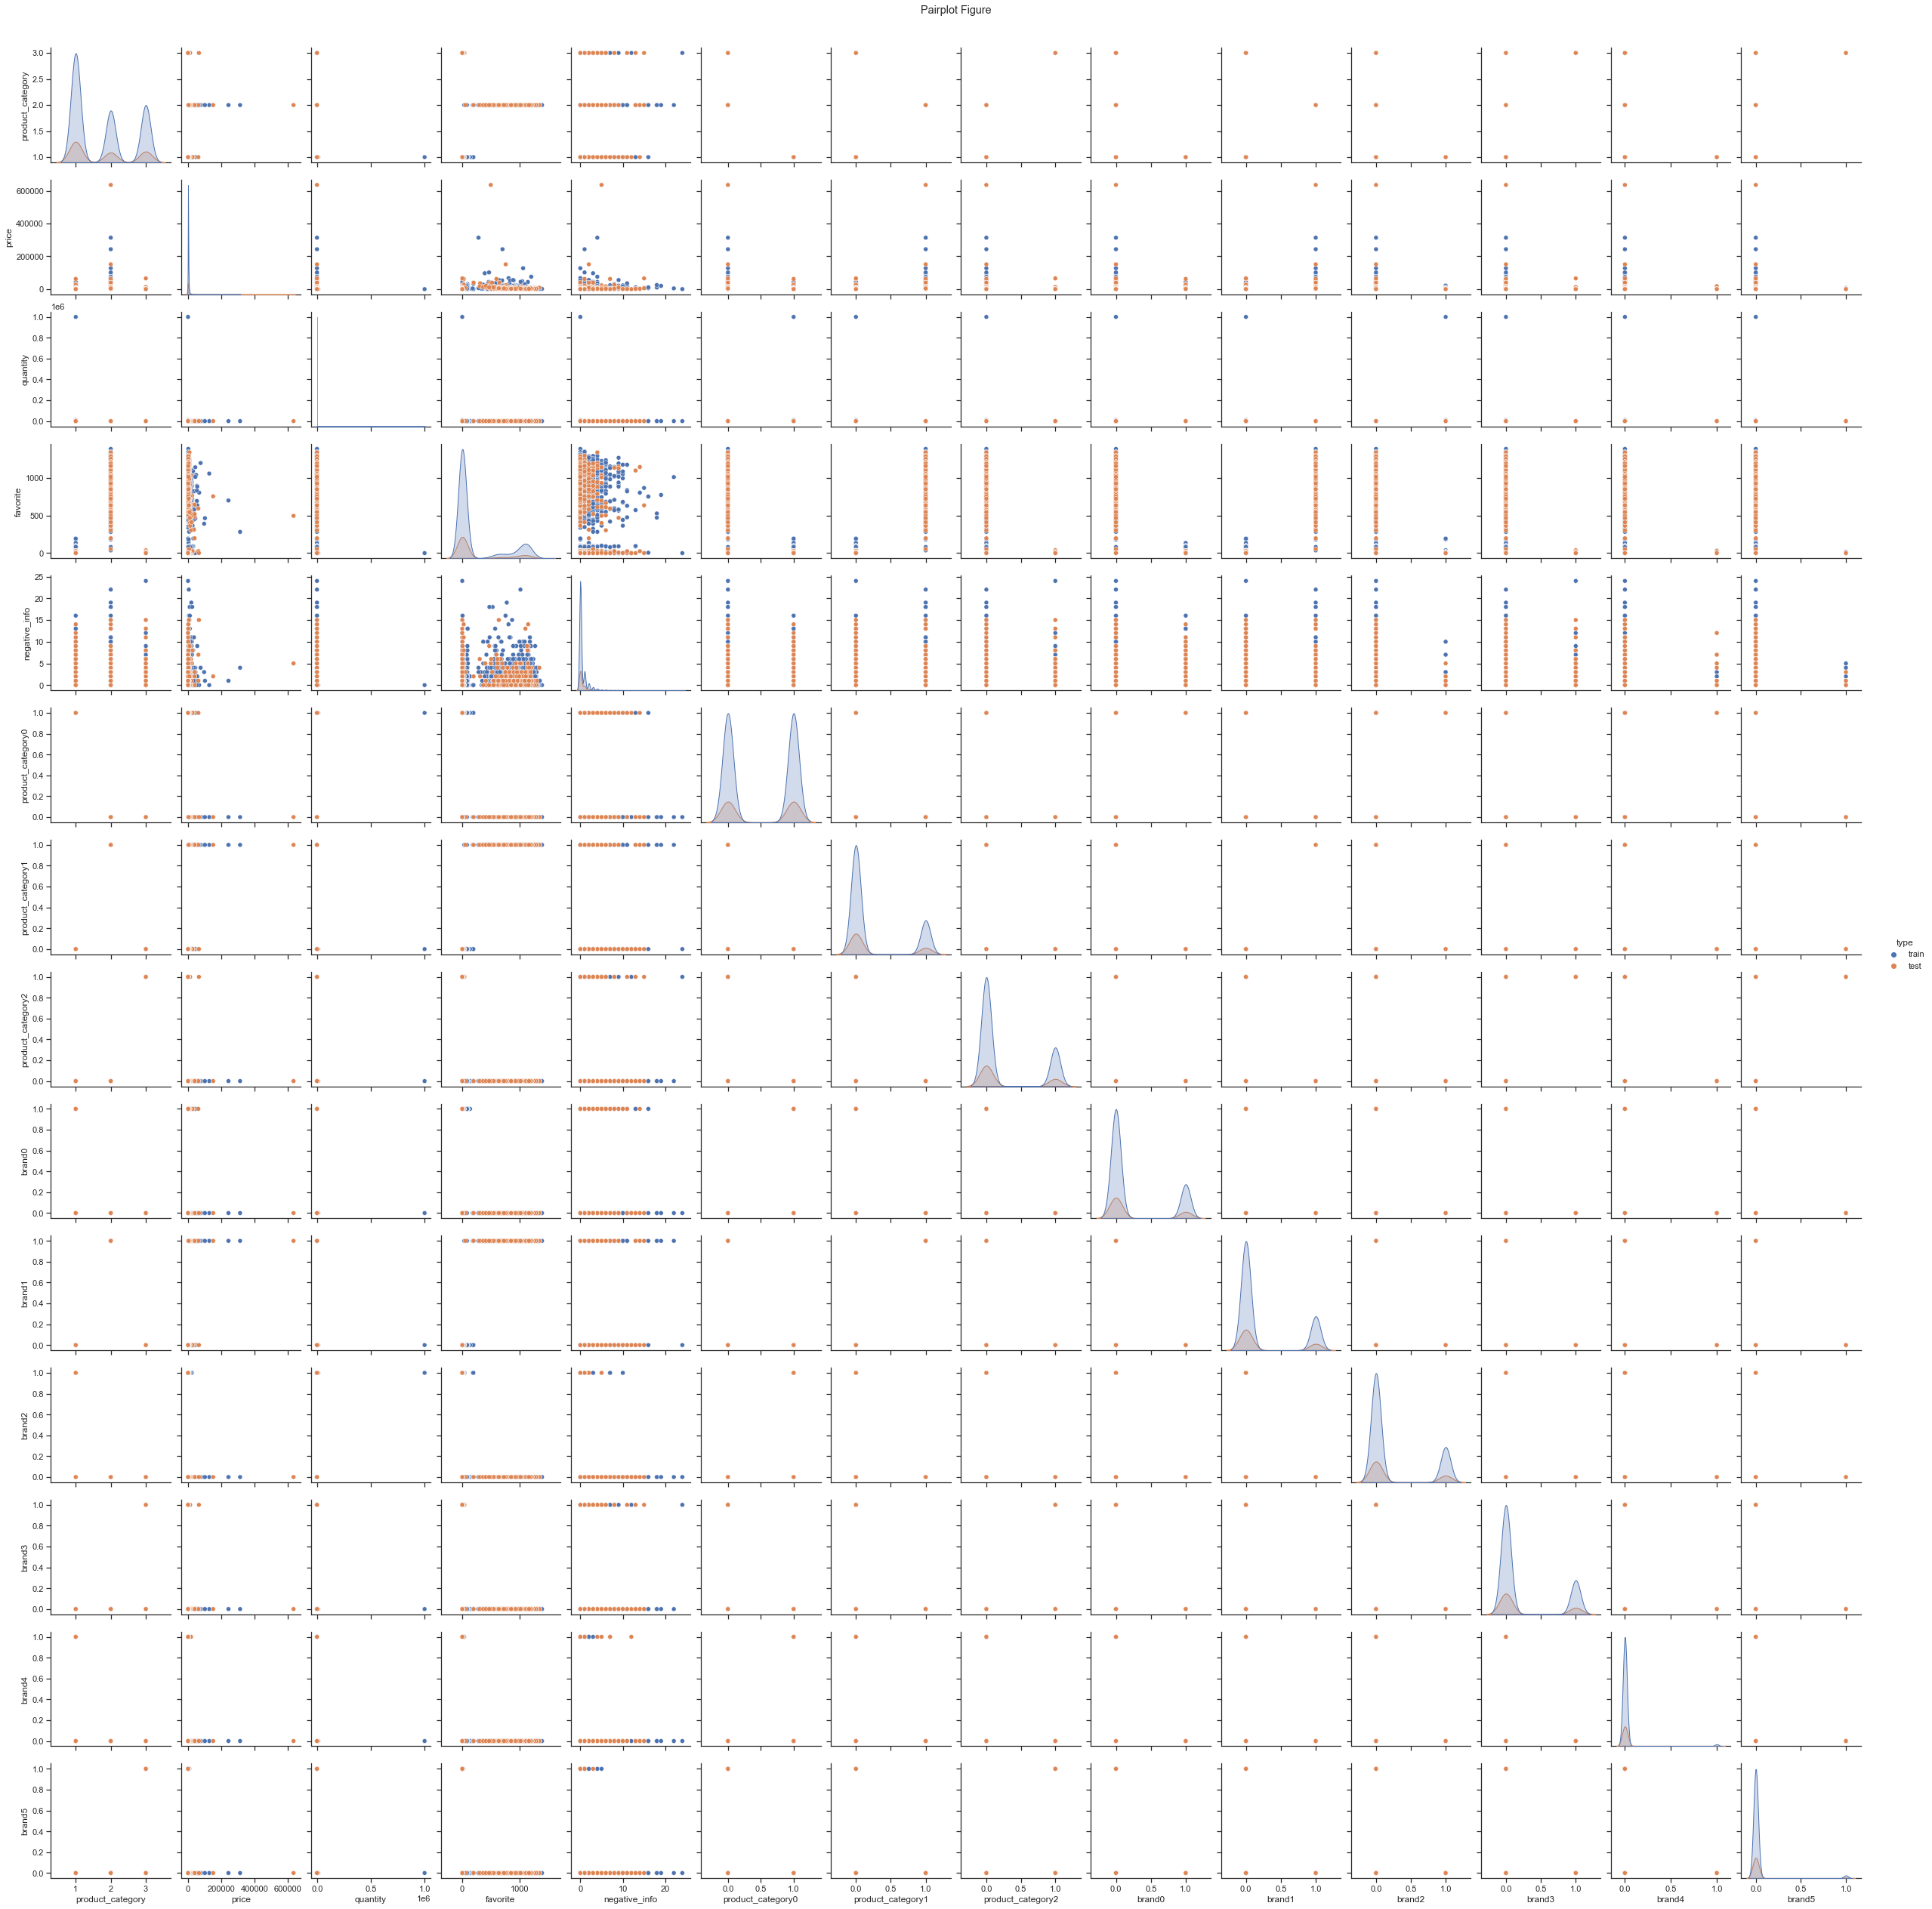
\includegraphics[width=0.45\linewidth]{figures/散点图矩阵}
	\caption{原始变量相关系数矩阵和散点图矩阵。相关系数矩阵中数字展示了相应行和相应列变量之间的相关系数,数值的绝对值越大,相关性越强。散点图矩阵中不同的颜色代表训练集和测试集,对角线绘制了该变量的核密度估计曲线。。}
	\label{fig:原变量相关系数矩阵}
\end{figure}
\par 利用散点图矩阵进一步展示各个变量之间的相关性,如图\ref{fig:原变量相关系数矩阵}。从图中可以看出价格和各个变量之间没有非常明显的关系,相对明显的是价格和负面评价数量之间,负面评价数量越多,价格越低,但这种相关关系也并非线性。

\section{预测方法}
\subsection{特征提取方法及特征描述}
使用人工提取和CNN神经网络自动提取两种方法。人工提取方法主要利用cv2库进行提取,提取了包括图片的哈里斯角点数量、人脸数量、人脸平均位置、人脸平均大小、关键点数量、文字区域数量、轮廓数量、HSV三阶矩共16条特征。CNN神经网络提取特征利用了迁移学习的方法:把训练完成的图片识别Resnet50神经网络\cite{Resnet50}中的最后两层进行改造,把图片按照价格高低分成20类,尝试对图片进行分类训练,重新训练完成的神经网络取最后一层fc层输出512维特征,作为CNN神经网络提取出来的特征。
\begin{figure}[!htbp]
	\centering
	\subfigure[原图]{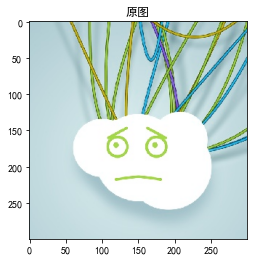
\includegraphics[width=0.40\linewidth]{哈里斯-原图}}
	\subfigure[操作后]{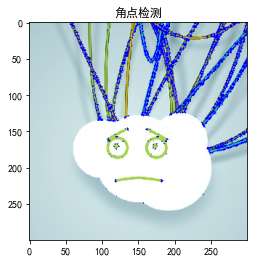
\includegraphics[width=0.4\linewidth]{哈里斯-操作}}
	\caption{哈里斯角点检测。图中展示了哈里斯角点的操作,左图均为原图,右图为识别之后的图片,图中蓝色区域即为识别之后的结果。图中边缘提取几乎都被检测出蓝点,可见哈里斯角点检测效果比较出色。}
	\label{图:人工特征}
\end{figure}

\begin{figure}[!htbp]
	\centering
	\subfigure[原图]{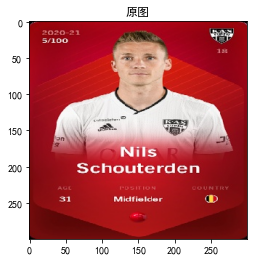
\includegraphics[width=0.4\linewidth]{人脸-原图}}
	\subfigure[操作后]{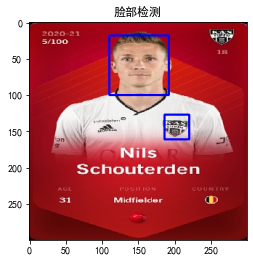
\includegraphics[width=0.4\linewidth]{人脸-操作}}
	\caption{人脸检测。图中展示了人脸检测的操作,左图为原图,右图为识别之后的图片,图中蓝色区域即为识别之后的结果。图中人脸被识别出两处,可见这种检测方法依然存在不完善之处。}
	\label{图:人工特征2}
\end{figure}
\par 在人工提取的特征中,主要使用了哈里斯角点检测等方法。哈里斯角点检测由哈里斯教授提出,属于早期的角点检测方法,主要描述如公式\ref{公式:哈里斯角点},其中$w(x,y)$是窗口函数,为下面的像素赋予权重,需要最大化后半部分位移强度,具体参见参考文献\cite{哈里斯角点}。哈里斯焦点检测的效果如图。人脸数量、人脸平均位置、人脸平均大小都是通过人脸检测的方法来完成,具体利用了基于级联的人脸检测方法,使用opencv提前训练好的数据\cite{opencv2022Jan},识别人脸数量、人脸平均位置和人脸平均大小等,检测效果如图\ref{图:人工特征}。关键点数量通过使用\cite{starkeypoint2008}中的算法进行,这个算法和哈里斯角点检测算法有较大的区别,作为评价图片的另一个纬度。文字区域数量通过轮廓检测的方法完成,通过查找满足一定条件的轮廓,检测出可能的文字区域,当然这种查找方法并不十分准确。轮廓检测可以检测出图片的轮廓数量。HSV三阶矩主要是通过HSV的算法进行操作,首先是利用转换函数将图片转换为HSV的格式,这种格式展示了图片的色调、饱和度和亮度,这符合人类的视觉,分别在H、S、V三个通道上计算一阶矩、二阶矩和三阶矩用以表示相应均值、方差和偏度。例如H计算了三阶矩分别表示了图片的平均色调,图片的色调的变化剧烈程度,图片色调是否是无偏的。
\begin{align}
	\begin{split}
		max \quad	E(u,v)=\sum_{x,y}w(x,y)\left[I(x+u,y+v)-I(x,y)\right]^2
	\end{split}
	\label{公式:哈里斯角点}
\end{align}
\par 机器学习的方法提取到了512维特征,由于这些特征维度高,没有公认的理论进行描述,在此只选择其中几个特征尝试进行描述。如图\ref{图:300}、\ref{图:392}和\ref{图:455},这些图都是选择了相应特征值最高的几张图片,其中图300中的特征为格纹以及缤纷的色彩,392和455特征为光柱和较为阴暗的面具图案。可见这些相同特征内部图片有着一定的共同点,不同特征之间的图片有较为显著的差异,机器学习方法提取特征总体来说较为合理。
\begin{figure}[!h]
	\centering
	\subfigure{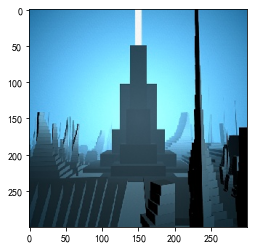
\includegraphics[width=0.28\linewidth]{392-1}}
	\subfigure{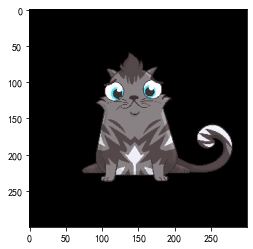
\includegraphics[width=0.28\linewidth]{392-2}}
	\subfigure{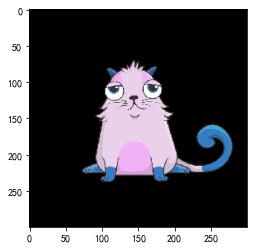
\includegraphics[width=0.28\linewidth]{392-3}}
	\subfigure{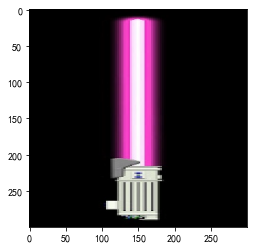
\includegraphics[width=0.28\linewidth]{392-4}}
	\subfigure{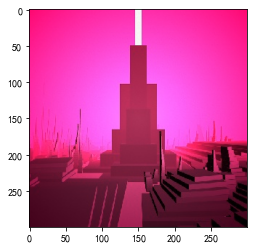
\includegraphics[width=0.28\linewidth]{392-5}}
	\subfigure{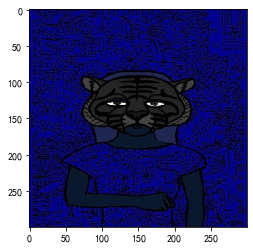
\includegraphics[width=0.28\linewidth]{392-6}}
	\caption{特征392图片展示。选择“392”特征数值偏高的图片进行展示。特征"392"偏高的图片给人一种深沉、压抑的感觉,背景以黑色或白色这种单调的色彩为主,色彩对比度不明显,“灰色光柱”和“黑色猫”是主要的图片。}
	\label{图:392}
\end{figure}
\begin{figure}[!h]
	\centering
	\subfigure{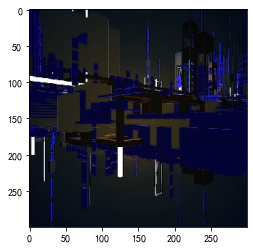
\includegraphics[width=0.28\linewidth]{455-1}}
	\subfigure{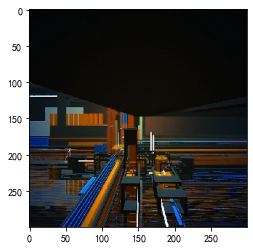
\includegraphics[width=0.28\linewidth]{455-2}}
	\subfigure{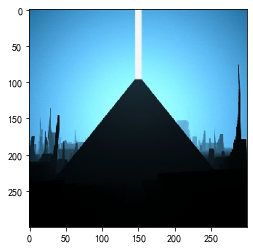
\includegraphics[width=0.28\linewidth]{455-3}}
	\subfigure{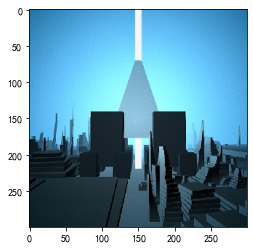
\includegraphics[width=0.28\linewidth]{455-4}}
	\subfigure{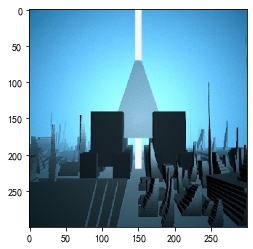
\includegraphics[width=0.28\linewidth]{455-5}}
	\subfigure{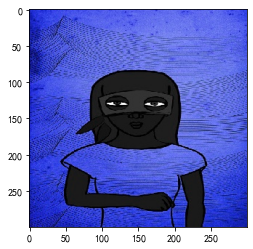
\includegraphics[width=0.28\linewidth]{455-6}}
	\caption{特征455图片展示。 特征“455”普遍选择了有、色调阴暗的图片,同时和392相比,还选择了线条更复杂的图像,比如发光的三角塔,还有蒙面女郎像。这些特征直观来看价格比较高,处于中位数以上。}
	\label{图:455}
\end{figure}
\begin{figure}[!h]
	\centering
	\subfigure{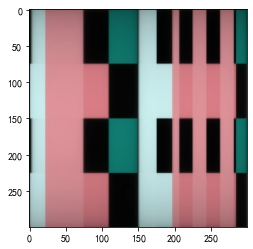
\includegraphics[width=0.28\linewidth]{300-1}}
	\subfigure{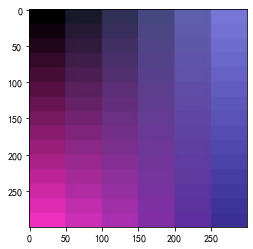
\includegraphics[width=0.28\linewidth]{300-2}}
	\subfigure{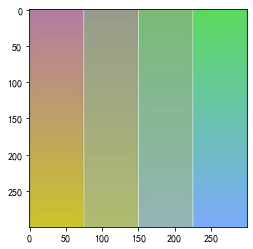
\includegraphics[width=0.28\linewidth]{300-3}}
	\caption{特征300图片展示。 特征“300”主要的特征是颜色上偏向于鲜艳、渐变、特征“300”高的图片在横竖分隔上只突出一个方向,要么突出横向,要么突出纵向。}
	\label{图:300}
\end{figure}
\par 由于数据维度过高,很难在此呈现所有数据的分布,取六个人工特征分析其分布情况,如图\ref{图:特征分布}。使用相关系数矩阵和调和曲线图给出数据之间相关性的分析,如图\ref{图:总特征矩阵},从相关系数矩阵中可以看出,特征之间有些存在不小的负相关情况,因此进行了一些删除操作;从调和曲线图可以看出,不同的价格区间之间有分开的特征组合点,其中价格区间1和其他价格之间的差别尤其大,说明这些特征有一定的合理性。
\begin{figure}[!htbp]
	\centering
	\subfigure{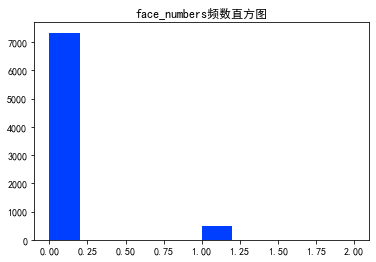
\includegraphics[width=0.28\linewidth]{face_numbers}}
	\subfigure{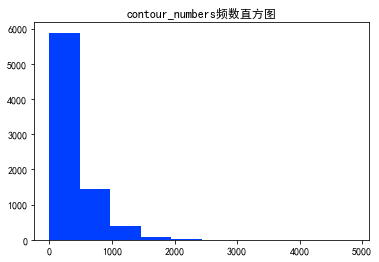
\includegraphics[width=0.28\linewidth]{contour_numbers}}
	\subfigure{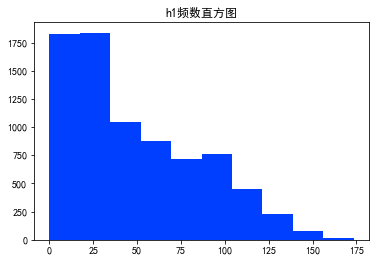
\includegraphics[width=0.28\linewidth]{h1}}
	\subfigure{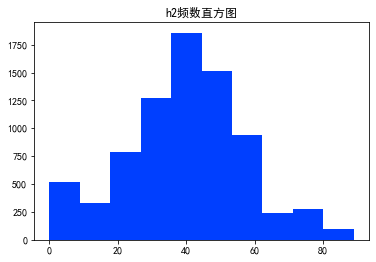
\includegraphics[width=0.28\linewidth]{h2}}
	\subfigure{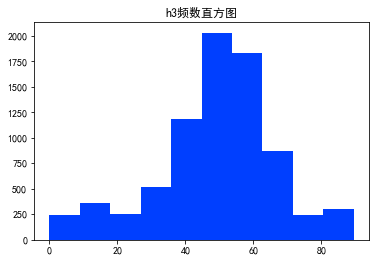
\includegraphics[width=0.28\linewidth]{h3}}
	\subfigure{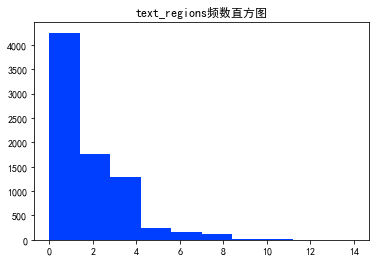
\includegraphics[width=0.28\linewidth]{text_region}}
	\caption{特征分布频数直方图。图中展示了六个频数分布直方图,其中不同的特征呈现不同的分布,脸部数量等呈现出右偏分布,h2,h3等呈现正态分布。}
	\label{图:特征分布}
\end{figure}
\begin{figure}[!htbp]
	\centering
	\subfigure{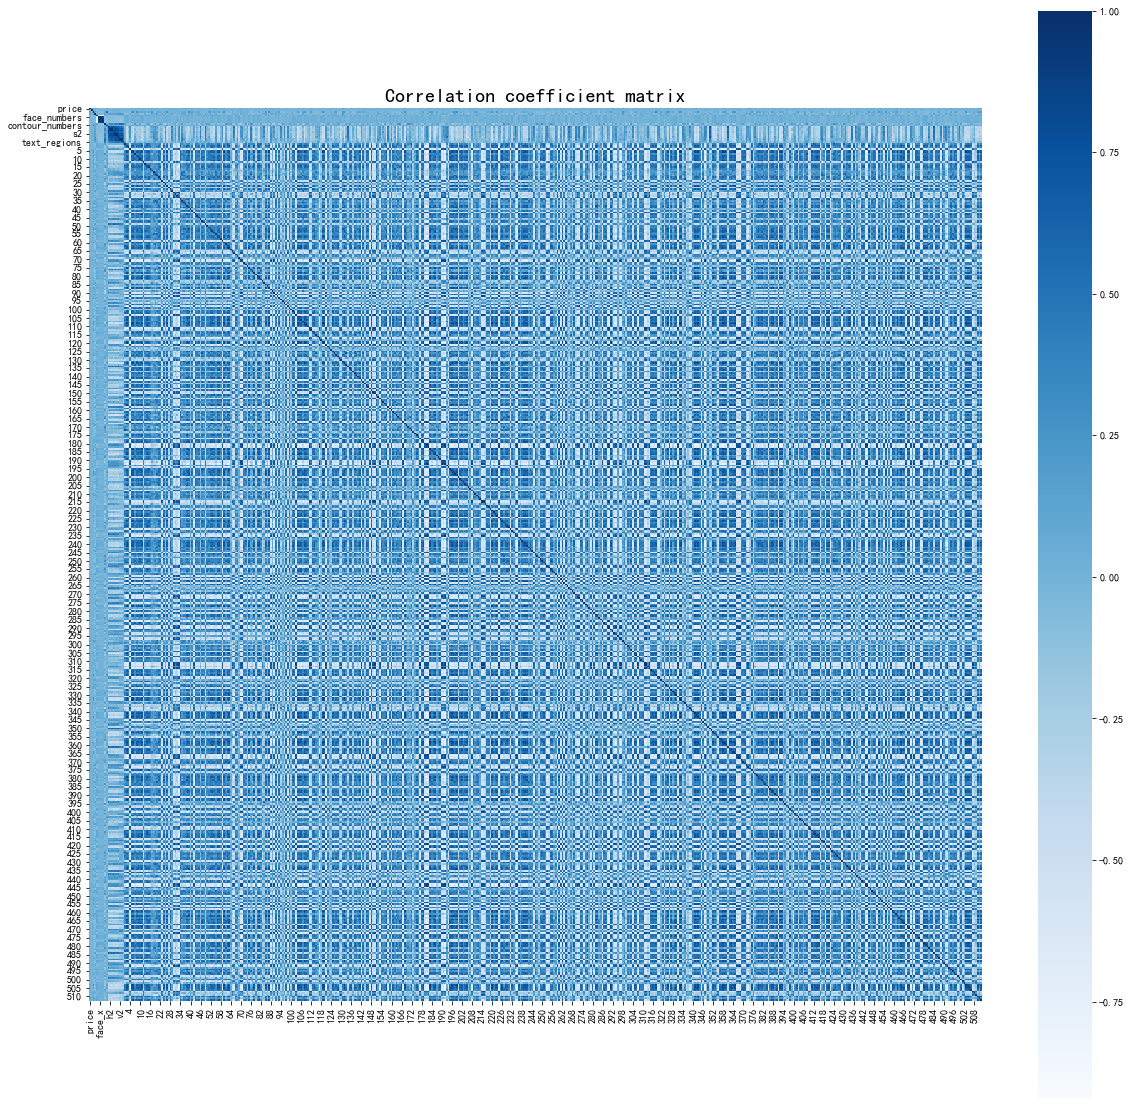
\includegraphics[width=0.45\linewidth]{所有变量相关系数矩阵}}
	\subfigure{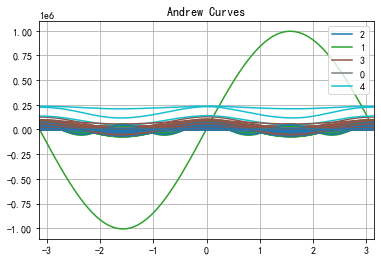
\includegraphics[width=0.45\linewidth]{调和曲线图}}
	\caption{总特征描述。相关系数矩阵按照颜色表示所有特征之间的相关性,白色代表相关系数为-1,深蓝色代表相关系数为+1。调和曲线图适用所有特征和所有变量绘制,价格范围按照四等分点对数据进行四等分获得。}
	\label{图:总特征矩阵}
\end{figure}

\subsection{预测模型构建}
选择广义线性模型、梯度提升树以及随机森林三个模型作为预测的价格候选模型,使用Gridsearch的方法选择合适的参数进行回归。在统计学中,广义线性模型(GLM)是对普通线性回归的一种灵活的概括。GLM通过允许线性模型通过一个链接函数与响应变量相关,并允许每个测量的方差大小成为其预测值的函数,从而对线性回归进行了推广\cite{ContributorstoWikimediaprojects2022Jan},但是广义线性回归仍然只是线性回归的变体,在复杂问题的预测精度上无法和其他模型相提并论,再次选用广义线性回归主要是作为其他模型的一种比较。梯度提升树和随机森林模型是基于树的回归模型,两者都是集成学习的典型代表。
使用GridSearch方法进行搜索,调整得到的最优参数如表\ref{tab:参数汇总}所示。
\begin{table}[!htpb]
	\centering 
	\begin{tabular}{|c|cc|}
		\hline 
		模型名称 & 参数名称 & 参数值 \\\hline 
		\multirow{2}{*}{广义线性模型} & 模型类型 & $gamma$\\  
		& 正则项 & 0.001 \\\hline 
		\multirow{3}{*}{GBT} & $maxIter$ & 30 \\
		& $maxDepth$ & 2\\
		& $minInfoGain$ & 0.0005\\\hline
		\multirow{2}{*}{RandomForest}
		& $maxDepth$ & 4\\
		& $numTrees$ &10 \\\hline 

	\end{tabular}
	\caption{参数汇总}
	\label{tab:参数汇总}
\end{table}

\section{结果分析及讨论}
选用MAE,RMSE,R2作为回归分析的主要指标进行评价。不同模型的结果如表\ref{tab:模型评价},其中线性模型表现最差,其在训练集和测试集的表现所有指标都不如另外两个模型,可见的性能明显低于其他回归方法的性能,在此验证了机器学习回归方法的必要性。
\begin{table}[!h]
	\centering
	\begin{tabular}{|c|ccc|ccc|}
		\hline
		\multirow{2}{*}{模型名称} &  \multicolumn{3}{c|}{训练集}       &  \multicolumn{3}{c|}{测试集}  \\
		\cline{2-7}
		&      MAE  &  RMSE     &    $R^2$   &   MAE     &   RMSE    &  $R^2$\\ 
		\hline 
		广义线性回归 & 631.68 & 4234.03 & 0.05 & 782.99 & 2942.41 & 0.06 \\	  \hline 
		梯度提升树& 626.60 & 4187.70 & 0.07 & 772.76 & 2838.34 & 0.13  \\	 \hline 
		随机森林 & 588.17 & 3878.18 & 0.20 & 746.75 & 2904.32 & 0.09 \\	 \hline  
	\end{tabular}
	\caption{模型评价}
	\label{tab:模型评价}
\end{table}
\par 另外,在另外两个树模型中,总体的表现互有优劣:GBT算法在训练集上表现不如随机森林,$R^2$为0.07,小于随机森林的0.2;RMSE和MAE表现为4187.70和626.60,不如随机森林的3878.18和588.17。而RandomForest在测试集上表现不如梯度提升树,$R^2$只达到了0.09,低于梯度提升树的0.13,在MAE和RMSE的表现上也不如梯度提升树。这说明梯度提升树和随机森林模型无法在这个问题上说明性能的好坏。另外梯度提升树的性能在这个问题上似乎表现也不稳定,主要在于$R^2$指标上,梯度提升树在训练集上的表现还不如测试集的表现。随机森林可能在这里出现了过拟合的问题,泛化性能还有待提升,同时也说明可能在这个问题上没有办法继续提升精度。
\par 整理各个模型的重要性如表\ref{tab:特征重要性}。favorite数量的重要性不言自明,但是也因此使得商家为了推高价格,故意购买水军、注册机器账号刷favorite指数等欺诈行为成为可能;哈里斯角点数量展示了图片本身的特点,当图片角点更多,可能说明了图片变化更加复杂,从而图片的价格更高,也就更受欢迎;特征“392”和特征“455”的描述已经在前文中进行过叙述,主要特征是色调偏向灰暗,对比度不高,以“光柱金字塔”、黑色宠物猫(黑色背景)以及灰色背景蒙面黑人为主,这些图片的价格高于大多数的商品,也可见有着灰暗色调、低对比度偏向深沉的图片更受欢迎,价格更高;产品类别2在图\ref{图:单变量-箱线图}中已经进行过展示,类别2平均价格普遍更高,可能是产品类别2的受众人群与众不同导致。
\begin{table}[!htpb]
	\centering
	\begin{tabular}{c|cc}
		\hline 
		特征名称  & GBT重要性 & RandomForest重要性\\\hline
		0(favorite) &  0.0667 & 0.1517 \\
		2(哈里斯角点数量) & 0.0333 & 0.0268 \\
		396("392"特征) & 0.0667 & 0.0062  \\
		455("455"特征) & 0.1 & 0.0019\\
		514(产品类别2) & 0.0333& 0.1055 \\\hline 
	\end{tabular}
	\caption{特征重要性排序。表中统计了GBT和RF中共同出现的元素,特征名称中括号外是向量化后的特征标号,括号内是对应的特征名称。}
	\label{tab:特征重要性}
\end{table}

\par 值得注意的是预测的结果并不准确,原因是多方面的。首先,NFT本身还不健全,存在着效率低下的问题\cite{Dowling2022Jan},即使使用了异常值检验的方法,依然无法保证排除了市场欺诈等行为;另外,模型的特征选择并不能完全反映市场状况,NFT市场中影响价格的因素是多方面的,而在NFT市场中的商品也未必可以成功出售出去,在这里只研究了成功出售的商品,没有不可以成功出售的商品,也就不能完整地反映市场总体的状况;最后,正如Dowling等人指出的那样,NFT市场中\cite{两页NFT价格预测}虽然买家对非功能性收藏品的估价与我们期望他们对实物收藏品的估价很相似,但卖家的定价往往不是最优的,这种机制的存在不是目前处理得到的图片特征等能够展现出来的,因此容易导致回归方法产生不准确的估价。
\par 另外,较低的预测准确率也说明了NFT本身市场效率偏低,如果市场能够达到较为完美的状态,那么随着图片本身的特征的客观因素变化,更容易得到预测性能准确,泛化性能良好的模型。正因此,NFT市场的定价机制还有待进一步研究,同时NFT市场本身也有待进一步发展。
\par 该研究存在一些局限性。可用的交易数量相对较少是一个明显的限制,尽管这是早期研究的普遍现象。在机器学习模型中没有考虑反映市场本身变化的情况,如不同的时间可能活跃用户数量不同,这对定价很重要。这种遗漏也是可用交易数量有限的一个因素。我们还可以考虑与更广泛的资产市场的联系,包括股票和债券市场。未来的研究中可以更加注重大环境,如将单一市场之外的市场与NFT联系起来。



% *** REFERENCES ***
\newpage
\bibliography{bibliography}
\bibliographystyle{naturemag}

\end{document}
